\documentclass[a4paper,11pt]{nurop}
\usepackage{amssymb}
\usepackage{mathbbold}
\usepackage{latexsym}
\usepackage{amsmath}
\usepackage{url}
\usepackage{graphicx}
\usepackage{amsthm}
\parindent=0in
\begin{document}
\author{\large{Bi Ran}\footnote{Student} and \large{Leong Tze Yun}\footnote{Supervisor}\\
	\normalsize\textit{Department of Computer Science,\\
	School of Computing,\\
	National University of Singapore}
}
\title{Hand Written Digit Recognition and Its Improvement}

\maketitle
\begin{abstract}
In this paper, two algorithms are compared on the task of handwritten digits recognition: C4.5 decision tree and support vector machine(SVM). Result shows that C4.5 has a poor performance, while pairwise C4.5 and boosted C4.5 performance much better; SVM has the best performance among these algorithms. A feature extracting method is proposed, which aims to improve classification performance by extract useful features manually. It is shown that performance of C4.5 and SVM has significant improvement on data set with new features added.
\end{abstract}
\section{Introduction}
 Handwritten digits recognition is a classic problem of machine learning. The objective is to recognize images of isolated handwritten digits(0-9). More specifically, the problem is equivalent to find a model, which takes image of handwritten digit as input, and output the predicted class label of the image. Model with prediction with high accuracy is preferred. In practice, different writing style, bad handwriting, and ambiguity among similar shaped digits make some images hard to recognize. Because different people have different writing style, and even the same person does not write two same characters in exactly the same way, building a recognition system which can recognize any character with good reliability in every application is impossible\cite{fabien06}.\\
 The first part of the paper compares the performance between C4.5, and SVM algorithms. Several techniques are applied to improve the performance of C4.5 and SVM. Semeion Handwritten Digit Data Set is used for training and testing in this paper. Considering the limited size of data set, cross-validation is used for performance evaluation. The second part introduces a method to improve classification performance by applying feature extraction. Extracted features are appended to the original data set. It will be shown that the feature extraction method not only improve performance of both C4.5 and SVM, but also generalize well on other handwritten digit data sets.
\section{Background and Motivation}
Handwritten digit recognition has important usage such as recognizing zip code and online recognition on computer tablets. Support vector machine and neural network are popular algorithms in this field, and impressive results has been achieved. In \cite{lecun98}, the author use artificially distorted examples to expand training set, and use convolutional neural network to do training and testing, which gives error rate less than 1\% on MNIST\footnote{a benchmark data set of images of segmented handwritten digits.} data set. In \cite{fabien06}, the author introduced a trainable feature extractor based on LeNet5 neural network, and use elastic distortion or affine transformations for the expansion of the training set, and achieved performance comparable to the best published result by using SVM algorithm.\\
In practice, ``reject'' is considered an allowed output when doing classification. For example, in case of zip code recognition, if the zip code of some letter is hard to recognize, then the letter can be rejected, and it will be send back to the sender. Sometimes, reject is preferred compared to misclassification. Consider that sending the letter back to the sender is much cheaper than sending it to a wrong place. Neural network has been applied on this situation, and the preference of ``reject'' and ``misclassification'' can be controlled by tunable threshold\cite{slg92}. In this paper, we do not consider ``reject'' case, and the our target is simply maximize the accuracy of classification.\\
Decision tree is a popular algorithm in data mining, while it is rarely used to do handwriting recognition. SVM is a relatively new algorithm in machine learning, and it is one the algorithm which is comparable to those state of art algorithms\cite{lecun98}.\\
It is interesting to study why decision tree does not work well in handwritten digit recognition, while SVM has good performance. Testing various method to improve performance of decision tree may help discover the limitation and potential of this algorithm.
\section{Data Set}
Semeion Handwritten Digit Data Set\cite{semeion} is used for training and testing in this paper. 1593 handwritten digits from around 80 persons were scanned. Each digit stretched in a rectangular box 16x16 in a gray scale of 256 values.Then each pixel of each image was scaled into a 0-1 value using a fixed threshold. Thus each instance in the data set consists of 256 0-1 value, and a class label(0-9).\\
Each person wrote all digits on a paper from 0 to 9 twice. They write digits in normal way int the first time(Figure 1), and in a fast way in the second time(Figure 2).\\
The order of the instances in the data set is shuffled before training and testing, because the label distribution of the original data set is not random.
\begin{figure}
\centering
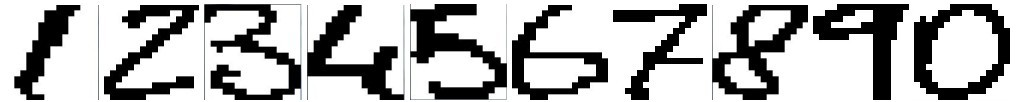
\includegraphics[width=1.0\textwidth]{clear}
\caption{written in normal way}
\end{figure}

\begin{figure}
\centering
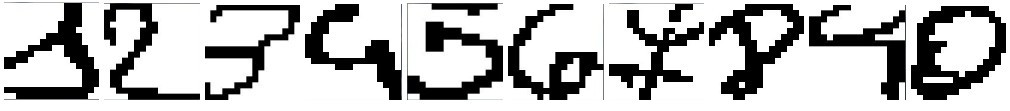
\includegraphics[width=1.0\textwidth]{unclear}
\caption{written in fast way}
\end{figure}

\section{Evaluation}

Because of the limited size of data set, we apply cross validation for evaluation purpose. Considering the trade-off between accuracy of estimation and time cost, we use 10-folds cross validation for performance evaluation, and compare the error rates of different algorithms.\\
In this paper, \emph{WEKA}\cite{weka} is used for all experiments on C4.5 decision tree. \emph{LIBSVM}\cite{libsvm} is used for training and testing support vector machine.\\
All source code, data set and modified data set is available at \url{http://code.google.com/p/cs2306-machine-learning/source/browse/#svn/trunk}.
\section{Experiment}
\subsection{C4.5}
Decision tree is a popular algorithm in data mining and machine learning. There are many decision tree algorithms, and we only consider C4.5 in this paper.\\
C4.5 is an improved version of ID3 decision tree. It follows a simple inductive bias: ``smaller trees are preferred'', which is motivated by Occan's Razor principle. To further simplify the decision tree to avoid over fitting problem, C4.5 perform pruning to limit the size of the tree. A pessimistic estimation of the error rate for each subtree is used when do the subtree replacement and subtree raising pruning in C4.5 algorithm. To achieve good performance, we perform parameter search on two tunable parameters: $C$ and $minObj$. $C$ is the confident factor, which is a threshold of the probability of the actual error rate being worse than the pessimistic estimation\cite{morgan.kaufmann}. Smaller confidence factor implies more pessimistic estimation, which will cause more drastic pruning. The $minObj$ is the minimum number of instances each leaf could have. Larger $minObj$ leads to smaller trees, which makes the tree more robust to noise.
\vspace{0.5cm}\\
\begin{tabular}{c|c c c c}
C$\backslash$ minObj	&1		&2		&3		&4\\
\hline \hline
1e-3 	&24.6077 \%	&24.3566 \%	&24.1682 \%	 &24.6704 \%\\
1e-2	&24.4193 \%	 &24.4821 \%	&24.231  \%	 &24.5449 \%\\
1e-1	&24.6077 \%	&24.231  \%	&24.231  \%	 &24.6077 \%\\
0.5 &24.2938 \%     &24.0427 \% &24.1055 \%  &24.8588 \%\\
1	&24.6077 \%	    &23.7916 \%	&24.1682 \%	 &24.796  \%\\
\end{tabular}
\vspace{0.5cm}\\

Test is performed on WEKA with all default parameter settings except $C$ and $minObj$. The result in the table above shows that he error rate of C4.5 algorithm is lowest(23.7916\%) when $C=1$ and $minObj=2$. It also shows that changing parameter has little influence on performance. This implies that pruning does not help much in this data set.\\
The performance of C4.5 is very poor compared to many other popular algorithms like support vector machine(will see it later). There are some possible reasons:\\
\begin{enumerate}
\item[1] Decision tree algorithm itself has limitation. The problem of learning optimal decision tree is NP-complete\cite{dtnpc}. C4.5 use a greedy algorithm to do searching, which does not guarantee to find the optimal decision tree.
\item[2] Although decision tree is able to estimate any discrete functions, some functions are harder to learn than others. For example, OXR function is hard to learn by decision tree, because the minimal decision tree for XOR requires a full binary tree , and it is hard to find ``small'' trees to estimate XOR well.
\item[3] Although C4.5 decision tree supports multi-class classification problem, more classes would result in larger trees. For example, assume there are $N$ classes, and each attribute is binary. Since each leaf can only represent one class, the height of the tree must be larger than $log_2(N)$. Thus the size of decision tree tends to become larger since the minimal possible tree size becomes larger. However, larger tree is opposed to Occan's Razor principle. Thus, C4.5 may not generalize well in multi-class classification problems.
\end{enumerate}
\subsubsection{Pairwise C4.5}
The first two reasons above are limitations of decision tree, which is hard to overcome. The third one can be overcame by converting multi-class classification problem into binary classification problem. Therefore, a large decision tree could be replaced by several small decision trees, which can be expected to have better generalization.\\
There are several methods to do this conversion, we only consider ``pairwise''(one-versus-one) method. Pairwise method train $N*(N-1)/2$ classifiers for each pair of classes(0/1,0/2,$\ldots$0/9,1/2,$\ldots$8/9). Unit for pair $i/j$ is trained only to classify class $i$ and $j$, thus it is only a binary classifier. When classifying a new instance, each classifier vote for the class based on their classification results. The class with the highest vote is considered as the classification result. If draw happens, the result is randomly chosen from those classes with the highest vote. Note that Pairwise C4.5 is equivalent to normal C4.5 in binary classification problem.\\
Weka itself does not support this conversion, so a separate program(using WEKA's library) is used to perform this test\footnote{Source code is available at \url{http://code.google.com/p/cs2306-machine-learning/source/browse/#svn/trunk/src}}.\\
\vspace{0.5cm}\\
\begin{tabular}{c c}
Algorithm	& Error rate\\
\hline \hline
normal C4.5	& 23.7916\%\\
Pairwise C4.5	& 15.5345\%\\
\end{tabular}
\vspace{0.5cm}\\
Pairwise C4.5 is implemented based on C4.5 algorithm implemented in WEKA's library with default parameter setting: $C=0.25,minObj=2$. We can see from the table that pairwise C4.5 performs much better than original C4.5. In pairwise C4.5, although there are more decision trees, the size of each tree is small(about 20 nodes per tree on average). However, the size of the tree for the original C4.5 is 293. Thus, pairwise C4.5 performs better since small trees are more likely to generalize well on unseen data.
\subsubsection{Boosted C4.5}
Boosting is an algorithm which aims to boost weak classifier into a strong classifier. The boosting algorithm used in this paper is AdaBoosting M1 provided in WEKA.\\
The boosting algorithm constructs the classifier by running several iterations. Each iteration obtains a classifier by a weighted data set, and the output of the final classifier is obtained by weighted sum of the results of all classifiers. After each iteration, data set is reweighted. Instances misclassified in the previous iteration has a larger weight so that they are more focused on in the future. The weight of each classifier is determined by their accuracy. Boosting works well with decision tree in practice, and it often does not suffer from over fitting problem.\\
Following result is obtained by applying boosting on C4.5 algorithm with different number of iterations.\\
\vspace{0.5cm}\\
\begin{tabular}{c c}
\# of Iterations	& Error rate\\
\hline \hline
	2		& 23.7916\%\\
	4		& 17.7024\%\\
	8		& 13.4965\%\\
	16		& 9.6673\%\\
    32      & 7.7841\%\\
    64      & 6.6541\%\\
\end{tabular}
\vspace{0.5cm}\\
Boosting is tested with WEKA's default parameter setting except for the number of iterations. From the table, we can see that the error rate drops when the number of iteration increases. Although further increase the number of iterations may obtain higher accuracy, the error rate would stop decreasing or start to increase(over fitting) at last.\\
Boosting algorithm constructs a classifier by combining several classifiers, which intuitively increase the complexity of the classifier. However, according to Occan's Razor principle, simpler classifiers tend to generalize better on unseen data. Boosting algorithm seems a contradict with Occan's Razor principle.\\
One possible explanation is that the complexity of boosting is not measured by the number of classifiers, but by the ``margin'' of the classifier.
In Boosting algorithm, each classifier vote for a class with its weight, and the class with the highest weight is the result of classification. The margin of an example is defined by the difference between weight of correct class, and the sum of all weights of incorrect class. The larger the margin is, the more confident the classification for this instance is. The boosting algorithm tend to maximize margin of instances, and convergence with some large margin distribution\cite{boosting}.\\
\subsubsection{Boosted Pairwise C4.5}
We can also apply boosting on Pairwise C4.5. The result is shown in the table below\footnote{Source code is available at \url{http://code.google.com/p/cs2306-machine-learning/source/browse/#svn/trunk/src}}\\
\vspace{0.5cm}\\
\begin{tabular}{c c c}
\# of Iterations	& Boosted C4.5 & Boosted Pairwise C4.5\\
\hline \hline
	2		& 23.7916\% & 15.283\%  \\
	4		& 17.7024\% & 12.075\%  \\
	8		& 13.4965\% & 9.3710\%  \\
	16		& 9.6673\%  & 8.0503\%  \\
    32      & 7.7841\%  & 6.8553\%\\
\end{tabular}
\vspace{0.5cm}\\
Boosted Pairwise C4.5 is implemented based on Pairwise C4.5 implemented above($C=0.25,minObj=2$), and AdaBoosting algorithm provided in WEKA's library(with default parameter setting). The result shows that boosted Pairwise C4.5 algorithm over performs boosted C4.5 algorithm. As mentioned above, pairwise C4.5 consists of multiple(45 in this case) decision trees. In Boosted Pairwise C4.5, the number of decision trees grows 45 times faster than boosted normal C4.5. However, Boosted Pairwise C4.5 turns out to have better performance, which support the argument ``the complexity of boosting is not measured by the number of classifiers''.

\subsection{Support Vector Machine}
Support vector machine(SVM) can be seen as a generalized version of linear classifier. SVM maps each instance into a higher dimensional feature space, and look for a hyperplane, which separate different classes. Hyperplane with large margin is preferred. All calculation of feature vectors with high dimension can be done efficiently via kernel function. Although new kernel functions are being purposed by researchers, four basic kernels are the most popular\cite{svm}:
\begin{itemize}
\item linear: $K(x_i,x_j)=x_i^Tx_j$\\
\item polynomial: $K(x_i,x_j)=(\gamma x_i^Tx_j+r)^d$, $\gamma >0$\\
\item radial basis function (RBF): $K(x_i,x_j)=\exp(-\gamma \|x_i-x_j\|^2)$, $\gamma > 0$\\
\item sigmoid: $K(x_i,x_j)=tanh(\gamma x_i^Tx_j+r)$\\
\end{itemize}
Here $\gamma$ and $r$ are kernel parameters.\\
According to \cite{ssk} and \cite{ll}, linear kernel is a special case of RBF kernel, and sigmoid kernel behaves like RBF kernel with certain parameters. Thus in this paper, we only consider RBF kernels.\\
There are many kinds of SVMs based on different error function. In this paper, we only consider C-svm, which minimize error function:
    $$\frac{1}{2}\|\vec{\beta}\|^2+C\sum_{i=1}^n \xi_i$$
 subject to:$$y_i(\vec{\beta}\cdot \vec{x_i}+\beta{0})\geq 1-\xi_i$$$$\forall i, \xi_i\geq 0$$

 We use grid-search\cite{svm} to find parameter with optimal performance: construct exponential growth sequence of $C$ and $\gamma$, and use cross validation for each $C$ and $\gamma$ to find a ``good'' region. More accurate grid search is performed on that region to find the optimal(locally) parameters. In this paper, tools provided in libsvm\cite{libsvm} package are used to perform the model selection procedure automatically.\\
As shown in Figure 3, the SVM tends to have the best performance when $C=2.0$ and $\gamma=0.0078125$, where the error rate is 4.2059\%.

Comparing to decision tree, SVM has much better performance on this data set. This is because in this data set, a instance consists of large amount of features(256 0-1 attributes), which makes it more likely to be linearly separable. In fact, SVM with linear kernel can achieve 0\% training error when classifying any digit against the rest in Semeion data set. This indicates that there exists a hyperplane which can separate any class from other classes. This also implies that all digits are pairwise separable. Moreover, SVM can find hyperplane gives the largest margin, which makes the classifier generalize well on unseen data. As it is shown that linear kernel is a special case of RBF kernel\cite{ssk,ll}, it is not surprising that SVM with RBF kernel has good performance on this data set.

\begin{figure}
\centering
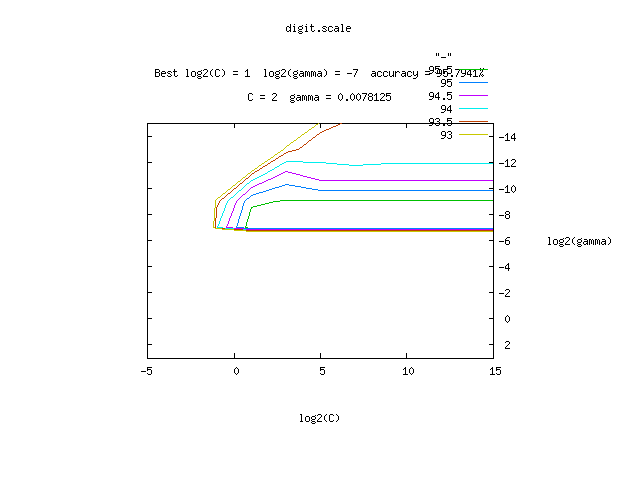
\includegraphics[width=1.0\textwidth]{digit}
\caption{grid search on $C,\gamma$}
\end{figure}

\section{Improvement}
\subsection{Motivation}
One observation from the algorithms is that neither decision tree nor SVM makes use of the information about the order of attributes. Actually, if some fixed permutation is applied on the attributes of each example in the data set, then decision tree and SVM will generate the same model as the model generated by original data set(subtle difference may exists, which depends on how the algorithm deals with ``tie conditions'', e.g. two attributes have the same information gain in C4.5). However, the positions of pixel are important for human when recognizing a image. Images also have strong 2-D local structure, pixels are correlated to pixels nearby\cite{lecun98}. If decision tree and SVM can make use of these information, their performance can be expected to have further improvement.\\

\subsection{Features Extraction}
One solution to this problem is to extract features which algorithms failed to capture. Feature extraction should be done before classification. In this paper, we extract several features derived from combination of pixels.\\
We add 16 extra features $r[16]$, one for each row, which describes how many ``black segments'' are there in the row. For example, in a image of ``1'', most of $r[i]$ can be expected to be $1$; in a image of ``0'', most $r[i]$ can be expected to be 2, and a few can be 1. Similarly, $c[16]$ are extracted for each column. The variance of the number of black pixels in each row and column are also added into each example. Thus, 34 extra features are extracted. These features are appended after each instance. The modified data set has 290 features.\\
\subsection{Testing and Analysis}
\vspace{0.5cm}
\begin{tabular}{c c c}
Algorithm		&	Original Data	&Modified Data\\
\hline \hline
C4.5                            &23.7916\%		& 18.5813\%\\
Pairwise C4.5                   &15.5345\%      & 12.3899\%\\
Boosted C4.5	                &7.7841\%		& 4.5198\%\\
Boosted PW C4.5	                &6.8553\%       & 5.2830\%\\
SVM                         	&4.2059\%       & 3.2643\%\\
\end{tabular}
\vspace{0.5cm}\\
The same training parameters as the earlier testing was used for each algorithm. From the result, we can see that all algorithms' error rates on modified data drops.\\
After sorting the all attributes by their information gain, 14 out of 15 features are newly added features. 21 out of total 34 new features ranks in top 30.\\
In the decision tree of the new data set, new features are made heavily used of. The size of the new tree is 229, which is smaller than the size of the tree of the old data set(293 nodes). Since smaller trees tends to generalize better, C4.5 can have better performance on the modified data set.\\

\subsection{Testing on MNIST Data set}
MNIST(\url{http://yann.lecun.com/exdb/mnist/}) is a popular handwritten digit data set. This data set contains 60000 instances for training, and 10000 instances for testing.  Similar to Semeion data set, instances in MNIST data set consists of 28*28 pixels of a image, each pixel is described by the gray scale of the pixel. To make time cost feasible, we make a random sample of 1800 instances from the training set for training. The whole testing data set(10000 instance) is used for testing. This is because testing is relatively fast compared to training, and large testing set would give closer estimation to the true accuracy. The range of feature in the original data set is 0 to 256, which is too large. We normalize attributes of instances to range from 0 to 1. This is to avoid attributes in greater numeric ranges dominate those in smaller numeric ranges. Another advantage is to avoid numerical difficulties when calculating vector inner product\cite{svm}. We do not need to normalize the Semeion data set because the range of features are between 0 and 1 initially. Grid search shows that $C=8, \gamma=0.0078125$ gives optimal(locally) performance.\\
Features with high information gain tends to have a more unbalanced separation of classes, which can help SVM find hyperplane with larger margins, thus lower complexity, and lower generalization error.\\
\vspace{0.5cm}
\begin{tabular}{c c c}
Algorithm	              & MNIST	& MNIST(with new features)\\
\hline \hline
C4.5                     & 26.66\%  & 19.99\%\\
Pairwise C4.5            &19.11\%   & 16.07\%\\
Boosted C4.5             & 8.79\%	& 7.58 \%\\
Boosted PW C4.5	         & 10.34\%  & 8.66 \%\\
SVM                      & 5.72\%   & 6.4\%\\
  \\
\end{tabular}
\vspace{0.5cm}\\
The error rate reduces as expected when adding extra features. Thus feature extraction can be expected to work on other image classification problems.\\

\section{Limitation Discussion}
The data set used in this paper is noise free, which means all instances are correctly labeled, and each pixel is mapped from corresponding region of image correctly. However, it may not be the case in reality situations. The noise resistance of learning algorithms is beyond the scope of this paper.\\
Memory usage is not considered in the comparison of algorithms because memory is usually considered less important than accuracy since the price of memory decreases fast. However, memory usage need to be considered when the dealing with large data set, or implementing algorithms directly on hardware.\\
Pairwise C4.5(and Boosted Pairwise C4.5) has better performance compared to normal C4.5(and boosted C4.5). However, the time cost for training and testing is several times longer. It turns out that in this C4.5 based algorithms, the algorithm with better performance tend to has longer training and test time. This trade off needs to be considered in piratical application.\\
Although feature extraction can improve classification performance, it can only extract small subset of information about pixel alignment and correlation data set. Large amount of information is still hidden inside the data set.\\
The size of data set is small compared to other similar data set. The accuracy can be expected to further improve by using a larger data set.\\
We only test feature extraction on C4.5 and SVM. The effect of feature extraction on other algorithms are yet to be studied.\\

\section{Further Work}
\begin{itemize}
 \item How Pairwise C4.5 performs on other multi-class classification problems compared to normal C4.5.
 \item Apply other method to build multi-class C4.5 from binary C4.5(e.g. one-versus-all).
 \item Find out more methods to extract features from image(e.g. corner, edge detection).
 \item Whether feature extraction can improve performance of other classification algorithms.
 \item Study classification algorithms which can automatically extract features of correlation of pixels(e.g. convolutional neural network\cite{lecun98}).
\end{itemize}

\section{Conclusion}
Comparing performance of different algorithms on on Semeion Data Set, C4.5 algorithm performs poorly, and adjusting parameters doesn't change the result much. Pairwise C4.5 performs better than C4.5. Boosted C4.5 and Boosted Pairwise C4.5 has a much better performance than C4.5. C-SVM with RBF kernel manages to reach 4.2059\% error rate after parameter search. By adding extracted features into the data set, the accuracy of all these algorithms improves, and SVM achieves the lowest error rate: 3.2643\%. Improvement of SVM is also observed on MNIST data set. We believe feature extraction is applicable on other handwriting recognition problems.

\newpage
\bibliographystyle{plain}
\bibliography{ref}
\end{document}
